\centerline{\bf \Huge Вторая МатДрака}

\problem{\textbf{1}} Найдите какое-нибудь такое девятизначное число $N$, состоящее из различных цифр, что среди всех чисел, получающихся из $N$ вычеркиванием семи цифр,
было бы не более одного простого.

\problem{\textbf{2}} $\dfrac{\left(19 \dfrac{1}{6}+43,75\right): \dfrac{5}{6}}{(13,3-11,5): 1 \dfrac{4}{6}}-\dfrac{\left(26,8-23 \dfrac{3}{7}\right): \dfrac{6}{35}}{0,5}$

\problem{\textbf{3}} Из Цветочного города в Солнечный ведёт шоссе
длиной 12 км. На втором километре этого шоссе расположен железнодорожный переезд, который три минуты закрыт и три минуты открыт и т. д., а на четвёртом и на шестом километрах
расположены светофоры, которые две минуты горят красным светом и три минуты — зелёным и т. д. Незнайка выезжает из Цветочного города в Солнечный в тот момент, когда переезд
только что закрылся, а оба светофора только что переключились на красный. За какое наименьшее время (в минутах) он сможет доехать до Солнечного города, не нарушая правил, если
его электромобиль едет по шоссе с постоянной скоростью (Незнайка не умеет ни тормозить, ни
увеличивать скорость)?


\problem{\textbf{4}} В папирусе Ринда (Древний Египет) среди прочих сведений содержатся разложения дробей в сумму дробей с числителем 1 , например,

$$
\dfrac{2}{73}=\dfrac{1}{60}+\dfrac{1}{219}+\dfrac{1}{292}+\dfrac{1}{x}
$$


Один из знаменателей здесь заменён буквой $x$. Найдите этот знаменатель.

\problem{\textbf{5}} Начальник записал несколько простых чисел, использовав ровно по одному
разу все цифры от 1 до 9. Сумма этих простых чисел оказалась равной 225. Можно ли, использовав ровно по одному разу те же цифры, записать несколько простых чисел так, чтобы
их сумма оказалась меньше?

\problem{\textbf{6}} На сколько сумма $2^2+4^2+6^2+\ldots+100^2$ больше суммы $1^2+3^2+5^2+\ldots+99^2 ?$

\problem{\textbf{7}} Сумму цифр шестизначного числа умножили на произведение его цифр. Получилось 390. Найдите хотя бы одно такое шестизначное число.

\problem{\textbf{8}} Сколько целых чисел от 378 до 2433 имеют сумму цифр, делящуюся
на 5?

\newpage

\hspace{3mm}

\problem{\textbf{9}} По кругу лежат 100 пирожков, из них 53 с капустой, а остальные — с рисом. Алексей знает, какие из них с чем, и хочет выбрать 67 подряд лежащих пирожков
так, чтобы среди них было ровно $k$ с капустой. При каких $k$ ему это гарантированно удастся сделать независимо от расположения пирожков? Приведите все возможные варианты.

\problem{\textbf{10}} Назовём натуральное число «примечательным»,
если все его цифры попарно различны и их сумма равна 18. Найдите сумму примечательных
чисел, не превосходящих 950.

\problem{\textbf{11}} По кругу сидят 100 человек. Некоторые из них —
рыцари, всегда говорящие правду, остальные — лжецы, которые всегда лгут. Для некоторого натурального числа $k < 100$ каждый из сидящих произнёс фразу: «Следующие $k$ людей,
сидящих за мной по часовой стрелке — лжецы». Чему могло быть равно число $k$?


\problem{\textbf{12}} На верхней грани кубика 3×3×3 к центральному квадрату 1×1 приклеили кубик 1×1×1. Как разделить получившуюся фигуру на 7 равных?

\problem{\textbf{13}} В турнире по шашкам участвовали ученики 10 и 11 классов.
Каждый сыграл с каждым один раз. За победу участник получал 2 очка, за ничью — 1 очко,
за проигрыш — 0 очков. Одиннадцатиклассников было в 10 раз больше, чем десятиклассников,
и они вместе набрали в 4,5 раза больше очков, нежели все десятиклассники. Сколько очков
набрал самый успешный десятиклассник?

\problem{\textbf{14}}Назовем число «замечательным», если оно имеет
ровно 4 различных натуральных делителя, причем среди них найдутся два таких, что ни один
не кратен другому. Сколько существует замечательных двузначных чисел?

\problem{\textbf{15}} Комплект косточек домино выложен в виде прямоугольника 8×7 клеток. Попробуйте определить, как расположены косточки?

\begin{center}
    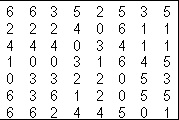
\includegraphics[width=0.4\textwidth]{Сборы/Сборы Элиста 2025/АА/7/91МатдракаII/Матдрака_15.png}
\end{center}